\documentclass[12pt, titlepage]{article}
\usepackage{xspace}
\usepackage{fullpage}
\usepackage[round]{natbib}
\usepackage{multirow}
\usepackage{booktabs}
\usepackage{tabularx}
\usepackage{graphicx}
\usepackage{float}
\usepackage{hyperref}
\hypersetup{
    colorlinks,
    citecolor=black,
    filecolor=black,
    linkcolor=red,
    urlcolor=blue
}

\newcommand{\li}[1]{\texttt{#1}\xspace}
%% Comments

\usepackage{color}

\newif\ifcomments\commentstrue

\ifcomments
\newcommand{\authornote}[3]{\textcolor{#1}{[#3 ---#2]}}
\newcommand{\todo}[1]{\textcolor{red}{[TODO: #1]}}
\else
\newcommand{\authornote}[3]{}
\newcommand{\todo}[1]{}
\fi

\newcommand{\wss}[1]{\authornote{blue}{SS}{#1}} 
\newcommand{\plt}[1]{\authornote{magenta}{TPLT}{#1}} %For explanation of the template
\newcommand{\an}[1]{\authornote{cyan}{Author}{#1}}

%% Common Parts

\newcommand{\progname}{FSL} % PUT YOUR PROGRAM NAME HERE %Every program
                                % should have a name


\newcounter{acnum}
\newcommand{\actheacnum}{AC\theacnum}
\newcommand{\acref}[1]{AC\ref{#1}}

\newcounter{ucnum}
\newcommand{\uctheucnum}{UC\theucnum}
\newcommand{\uref}[1]{UC\ref{#1}}

\newcounter{mnum}
\newcommand{\mthemnum}{M\themnum}
\newcommand{\mref}[1]{M\ref{m:#1}}

\begin{document}

\title{Module Guide for \progname} 
\author{Bo Cao}
\date{\today}

\maketitle

\pagenumbering{roman}

\section{Revision History}

\begin{tabularx}{\textwidth}{p{3cm}p{2cm}X}
\toprule {\bf Date} & {\bf Version} & {\bf Notes}\\
\midrule
Date 1 & 1.0 & Notes\\
Date 2 & 1.1 & Notes\\
\bottomrule
\end{tabularx}

\newpage

\section{Reference Material}

This section records information for easy reference.

\subsection{Abbreviations and Acronyms}

\renewcommand{\arraystretch}{1.2}
\begin{tabular}{l l} 
  \toprule		
  \textbf{symbol} & \textbf{description}\\
  \midrule 
  AC & Anticipated Change\\
  DAG & Directed Acyclic Graph \\
  M & Module \\
  MG & Module Guide \\
  OS & Operating System \\
  R & Requirement\\
  SC & Scientific Computing \\
  SRS & Software Requirements Specification\\
  \progname & Explanation of program name\\
  UC & Unlikely Change \\
  \wss{etc.} & \wss{...}\\
  \bottomrule
\end{tabular}\\

\newpage

\tableofcontents

\listoftables

\listoffigures

\newpage

\pagenumbering{arabic}

\section{Introduction}

Decomposing a system into modules is a commonly accepted approach to developing
software.  A module is a work assignment for a programmer or programming
team~\citep{ParnasEtAl1984}.  We advocate a decomposition
based on the principle of information hiding~\citep{Parnas1972a}.  This
principle supports design for change, because the ``secrets'' that each module
hides represent likely future changes.  Design for change is valuable in SC,
where modifications are frequent, especially during initial development as the
solution space is explored.  

Our design follows the rules layed out by \citet{ParnasEtAl1984}, as follows:
\begin{itemize}
\item System details that are likely to change independently should be the
  secrets of separate modules.
\item Each data structure is implemented in only one module.
\item Any other program that requires information stored in a module's data
  structures must obtain it by calling access programs belonging to that module.
\end{itemize}

After completing the first stage of the design, the Software Requirements
Specification (SRS), the Module Guide (MG) is developed~\citep{ParnasEtAl1984}. The MG
specifies the modular structure of the system and is intended to allow both
designers and maintainers to easily identify the parts of the software.  The
potential readers of this document are as follows:

\begin{itemize}
\item New project members: This document can be a guide for a new project member
  to easily understand the overall structure and quickly find the
  relevant modules they are searching for.
\item Maintainers: The hierarchical structure of the module guide improves the
  maintainers' understanding when they need to make changes to the system. It is
  important for a maintainer to update the relevant sections of the document
  after changes have been made.
\item Designers: Once the module guide has been written, it can be used to
  check for consistency, feasibility and flexibility. Designers can verify the
  system in various ways, such as consistency among modules, feasibility of the
  decomposition, and flexibility of the design.
\end{itemize}

The rest of the document is organized as follows. Section
\ref{SecChange} lists the anticipated and unlikely changes of the software
requirements. Section \ref{SecMH} summarizes the module decomposition that
was constructed according to the likely changes. Section \ref{SecConnection}
specifies the connections between the software requirements and the
modules. Section \ref{SecMD} gives a detailed description of the
modules. Section \ref{SecTM} includes two traceability matrices. One checks
the completeness of the design against the requirements provided in the SRS. The
other shows the relation between anticipated changes and the modules. Section
\ref{SecUse} describes the use relation between modules.

\section{Anticipated and Unlikely Changes} \label{SecChange}

This section lists possible changes to the system. According to the likeliness
of the change, the possible changes are classified into two
categories. Anticipated changes are listed in Section \ref{SecAchange}, and
unlikely changes are listed in Section \ref{SecUchange}.

\subsection{Anticipated Changes} \label{SecAchange}

Anticipated changes are the source of the information that is to be hidden
inside the modules. Ideally, changing one of the anticipated changes will only
require changing the one module that hides the associated decision. The approach
adapted here is called design for change.
\newcommand{\acitem}[1]{\item[\refstepcounter{acnum} \actheacnum \label{ac:#1}:] }
\begin{description}
\acitem{HardwareOS} The specific hardware and OS on which the software is running.
\acitem{Conversion} The format of the data that the conversion functions accept.
\acitem{FunctionType} The type used in the API's languages that represents a function transformed into a CFS.
\acitem{LinearSolver} The linear solver used in the division operation.
\acitem{Integral} The integral function used in transformation to CFS.
\end{description}

\subsection{Unlikely Changes} \label{SecUchange}

The module design should be as general as possible. However, a general system is
more complex. Sometimes this complexity is not necessary. Fixing some design
decisions at the system architecture stage can simplify the software design. If
these decision should later need to be changed, then many parts of the design
will potentially need to be modified. Hence, it is not intended that these
decisions will be changed.
\newcommand{\ucitem}[1]{\item[\refstepcounter{ucnum} \uctheucnum \label{uc:#1}:] }
\begin{description}
	\ucitem{DataStruct} The data structure to store $A_i$'s and $B_i$'s in the CFS's.
\end{description}

\section{Module Hierarchy} \label{SecMH}

This section provides an overview of the module design. Modules are summarized
in a hierarchy decomposed by secrets in Table \ref{TblMH}. The modules listed
below, which are leaves in the hierarchy tree, are the modules that will
actually be implemented.
\newcommand{\mitem}[1]{\item [\refstepcounter{mnum} \mthemnum \label{m:#1}:] }
\begin{description}
\mitem{BasicEnv} The module that provides basic functions. Part of the implementing languages' runtime libraries.
\mitem{LinearSolver} The linear solver module, implemented by others, and used by our library's division operation.
\mitem{Integral} The integral module, implemented by others, and used by the function in our library that transforms a mathematical function to a CFS.
\mitem{DataDef} The data definition module. 
\mitem{Conversion} The conversion module to convert other data formats from/to CFS's.
\mitem{Transformation} The transformation module to transform mathematical functions from/to CFS's
\mitem{BasicOp} The basic operation module including the addition, subtraction, multiplication, division and amplitude operation.
\mitem{AdvancedOp} The advanced operation module including the function of CFS, and tolerated equality operations.
\end{description}


\begin{table}[h!]
\centering
\begin{tabular}{p{0.3\textwidth} p{0.6\textwidth}}
\toprule
\textbf{Level 1} & \textbf{Level 2}\\
\midrule

{Hardware-Hiding Module} & \mref{BasicEnv} Basic functions module \\
\midrule

\multirow{7}{0.3\textwidth}{Behaviour-Hiding Module} 
& \mref{DataDef} Data definition module\\
& \mref{Conversion} Conversion module\\
& \mref{Transformation} Transformation module\\
& \mref{BasicOp} Basic operations module\\
& \mref{AdvancedOp} Advanced operations module\\
\midrule

\multirow{3}{0.3\textwidth}{Software Decision Module} 
& \mref{LinearSolver} Linear solver (external)\\
& \mref{Integral} Integral (external)\\
\bottomrule

\end{tabular}
\caption{Module Hierarchy}
\label{TblMH}
\end{table}

\section{Connection Between Requirements and Design} \label{SecConnection}

The design of the system is intended to satisfy the requirements developed in
the SRS. In this stage, the system is decomposed into modules. The connection
between requirements and modules is listed in Table \ref{TblRT}.

\section{Module Decomposition} \label{SecMD}

Modules are decomposed according to the principle of ``information hiding''
proposed by \citet{ParnasEtAl1984}. The \emph{Secrets} field in a module
decomposition is a brief statement of the design decision hidden by the
module. The \emph{Services} field specifies \emph{what} the module will do
without documenting \emph{how} to do it. For each module, a suggestion for the
implementing software is given under the \emph{Implemented By} title. If the
entry is \emph{OS}, this means that the module is provided by the operating
system or by standard programming language libraries.  \emph{\progname{}} means the
module will be implemented by the \progname{} software.

Only the leaf modules in the hierarchy have to be implemented. If a dash
(\emph{--}) is shown, this means that the module is not a leaf and will not have
to be implemented.

\subsection{Basic functions module (\mref{BasicEnv})}

\begin{description}
\item[Secrets:]The basic data structure and algorithm used to implement the library.
\item[Services:]Serves as the basic functions and data structure used by the rest of the
  system. This module provides the interface between the hardware, the OS and the
  software. So, the system can use it to build data structures, perform operations related to basic data types, display outputs or to accept inputs.
\item[Implemented By:] OS and run-time library of our implementing language.
\end{description}
\subsection{Software Decision Modules}
\subsubsection{Linear solver module \mref{LinearSolver}}

\begin{description}
\item[Secrets:]A linear equation solver.
\item[Services:]Solves the linear equation generated by \progname.
\item[Implemented By:] Third party.
\end{description}
\subsubsection{Integral module \mref{Integral}}

\begin{description}
	\item[Secrets:]A function that implements the integral of a function on a given interval.
	\item[Services:]Calculates the integration in the transformation from a mathematical function to its CFS.
	\item[Implemented By:] Third party
\end{description}

\subsection{Behaviour-hiding modules}
\subsubsection{Data definition module \mref{DataDef}}
\begin{description}
\item[Secrets:] Define the computational data structure of a CFS 
\item[Services:] Provide CFS's getters and setters.
\item[Implemented By:] \progname
\end{description}
\subsubsection{Conversion module \mref{Conversion}}
\begin{description}
	\item[Secrets:] Stores passed-in data in a CFS, and writes data in a CFS to user-designated spaces.
	\item[Services:] Provide conversion from/to data in other formats. 
	\item[Implemented By:] \progname
\end{description}
\subsubsection{Transformations \mref{Transformation}}
\begin{description}
	\item[Secrets:] Task1: Calculate the $A_i$'s and $B_i$'s in a CFS with given mathematical function $f(t)$, $n$, and $\omega$, and store $n$, $\omega$, $A_i$'s and $B_i$'s in a CFS. \\
	Task2: Calculate function values based on variable values and function's CFS.
	\item[Services:] Provide transformation from/to a mathematical function.
	\item[Implemented By:] \progname
\end{description}
\subsubsection{Basic operation \mref{DataDef}}
\begin{description}
	\item[Secrets:] Calculate the $A_i$'s and $B_i$'s for results of addition, subtraction, multiplication, and division operations, and calculate the result of amplitude operation. 
	\item[Services:] Provide addition, subtraction, multiplication, division and amplitude operations.
	\item[Implemented By:] \progname
\end{description}
\subsubsection{Advanced operation \mref{DataDef}}
\begin{description}
	\item[Secrets:] Calculate the $A_i$'s and $B_i$'s for functions of CFS's, and calculate the result of tolerated equality operation. 
	\item[Services:] Provide function of CFS and tolerated equality operations.
	\item[Implemented By:] \progname
\end{description}

\section{Traceability Matrix} \label{SecTM}

This section shows two traceability matrices: between the modules and the
requirements and between the modules and the anticipated changes.

% the table should use mref, the requirements should be named, use something
% like fref
\begin{table}[H]
\centering
\begin{tabular}{p{0.2\textwidth} p{0.6\textwidth}}
\toprule
\textbf{Req.} & \textbf{Modules}\\
\midrule
R1 & \mref{mHH}, \mref{mInput}, \mref{mParams}, \mref{mControl}\\
R2 & \mref{mInput}, \mref{mParams}\\
R3 & \mref{mVerify}\\
R4 & \mref{mOutput}, \mref{mControl}\\
R5 & \mref{mOutput}, \mref{mODEs}, \mref{mControl}, \mref{mSeqDS}, \mref{mSolver}, \mref{mPlot}\\
R6 & \mref{mOutput}, \mref{mODEs}, \mref{mControl}, \mref{mSeqDS}, \mref{mSolver}, \mref{mPlot}\\
R7 & \mref{mOutput}, \mref{mEnergy}, \mref{mControl}, \mref{mSeqDS}, \mref{mPlot}\\
R8 & \mref{mOutput}, \mref{mEnergy}, \mref{mControl}, \mref{mSeqDS}, \mref{mPlot}\\
R9 & \mref{mVerifyOut}\\
R10 & \mref{mOutput}, \mref{mODEs}, \mref{mControl}\\
R11 & \mref{mOutput}, \mref{mODEs}, \mref{mEnergy}, \mref{mControl}\\
\bottomrule
\end{tabular}
\caption{Trace Between Requirements and Modules}
\label{TblRT}
\end{table}

\begin{table}[H]
\centering
\begin{tabular}{p{0.2\textwidth} p{0.6\textwidth}}
\toprule
\textbf{AC} & \textbf{Modules}\\
\midrule
\acref{acHardware} & \mref{mHH}\\
\acref{acInput} & \mref{mInput}\\
\acref{acParams} & \mref{mParams}\\
\acref{acVerify} & \mref{mVerify}\\
\acref{acOutput} & \mref{mOutput}\\
\acref{acVerifyOut} & \mref{mVerifyOut}\\
\acref{acODEs} & \mref{mODEs}\\
\acref{acEnergy} & \mref{mEnergy}\\
\acref{acControl} & \mref{mControl}\\
\acref{acSeqDS} & \mref{mSeqDS}\\
\acref{acSolver} & \mref{mSolver}\\
\acref{acPlot} & \mref{mPlot}\\
\bottomrule
\end{tabular}
\caption{Trace Between Anticipated Changes and Modules}
\label{TblACT}
\end{table}

\section{Use Hierarchy Between Modules} \label{SecUse}

In this section, the uses hierarchy between modules is
provided. \citet{Parnas1978} said of two programs A and B that A {\em uses} B if
correct execution of B may be necessary for A to complete the task described in
its specification. That is, A {\em uses} B if there exist situations in which
the correct functioning of A depends upon the availability of a correct
implementation of B.  Figure \ref{FigUH} illustrates the use relation between
the modules. It can be seen that the graph is a directed acyclic graph
(DAG). Each level of the hierarchy offers a testable and usable subset of the
system, and modules in the higher level of the hierarchy are essentially simpler
because they use modules from the lower levels.

\begin{figure}[H]
\centering
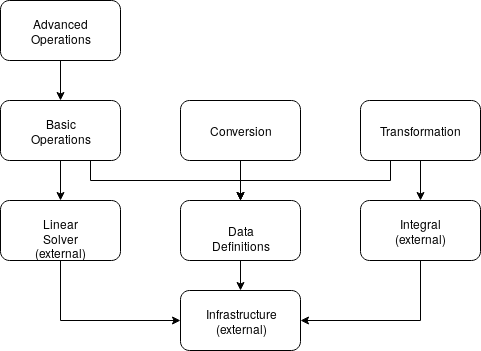
\includegraphics[width=0.7\textwidth]{UsesHierarchy.png}
\caption{Use hierarchy among modules}
\label{FigUH}
\end{figure}

%\section*{References}

\bibliographystyle {plainnat}
\bibliography{../../../refs/References}

\end{document}